Resumen de las principales características de las variables relevantes en los registros de logs de navegación.
Análisis de la distribución de los datos, incluyendo medidas de centralidad y dispersión. Haciendo uso de la librería pandas, de Python, podemos obtener informacion importante de los conjuntos de datos, estos valores nos proporcionarán un mayor entendimiento de la composición y estructura de los registros de navegación.

Podemos obtener informacion respecto a la cantidad de valores faltantes de cada dataframe que se está utilizando, los cuales son \textbf{36853} en total. En los dos primeros conjuntos de datos, no hay valores faltantes, y los 36,853 corresponden principalmente al campo 'canal', con solo un valor faltante en el campo 'método'. Haciendo uso de la misma librería, podemos determinar los tipos de datos que contiene cada campo. Es importante mencionar que los tres marcos de datos (dataframes) poseen la misma estructura, pero se detallará el contenido de cada uno por separado:
\begin{itemize}
    \item \textbf{rut cliente:} Contiene datos de tipo int64.
    \item \textbf{fecha evento:} Contiene datos de tipo object.
    \item \textbf{metodo:} Contiene datos de tipo object.
    \item \textbf{canal:} Contiene datos de tipo object.
\end{itemize}

Además se puede conocer la cantidad de valores únicos que posee cada una de las columnas de los 3 datasets:

Dataset 1:

\begin{itemize}
    \item \textbf{rut cliente:} Contiene 40125 valores únicos.
    \item \textbf{fecha evento:} Contiene 80181 valores únicos.
    \item \textbf{metodo:} Contiene 1 valor único.
    \item \textbf{canal:} Contiene 2 valores únicos.
\end{itemize}

Dataset 2:

\begin{itemize}
    \item \textbf{rut cliente:} Contiene 40224 valores únicos.
    \item \textbf{fecha evento:} Contiene 80470 valores únicos.
    \item \textbf{metodo:} Contiene 1 valor únicos.
    \item \textbf{canal:} Contiene 2 valores únicos.
\end{itemize}

Dataset 3:

\begin{itemize}
    \item \textbf{rut cliente:} Contiene 35541 valores únicos.
    \item \textbf{fecha evento:} Contiene 403325 valores únicos.
    \item \textbf{metodo:} Contiene 99 valores únicos.
    \item \textbf{canal:} Contiene 4 valores únicos.
\end{itemize}

%\begin{figure}[H]
    %\begin{minipage}[t]{0.9\textwidth}
        %\caption{Datos faltantes dataframes.}
        %\label{descripcion_dataframe}        
    %\end{minipage}

    %\vspace{10pt}

    %\begin{minipage}[b]{0.85\textwidth}
        %\centering
        %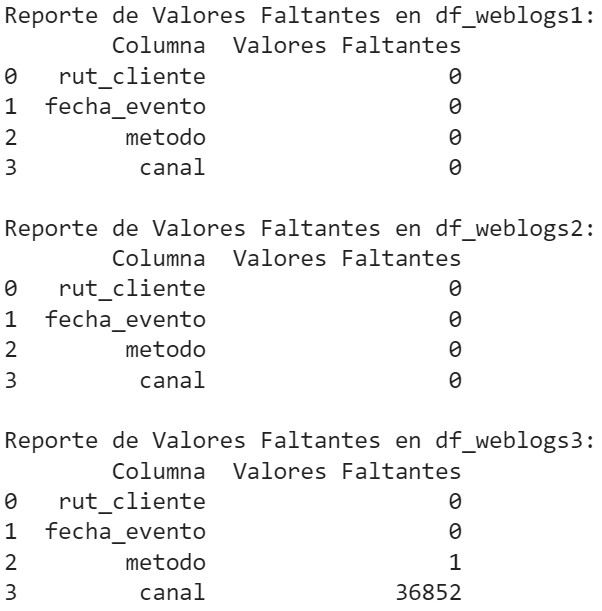
\includegraphics[width=\textwidth]{img/valores faltantes datasets.jpg}        
    %\end{minipage}

    %\begin{minipage}[t]{0.9\textwidth}
        %Fuente: Elaboración propia.
    %\end{minipage}
%\end{figure}

%Identificación de cualquier valor atípico o dato faltante en los registros y discusión sobre cómo se manejarán estos casos.